
\section{Sample growth}

The samples were grown and initially characterised by Prof. Takeuchi's group in Sendai University, Japan in May 2009 using the floating zone technique. Here powders of the correct stoichiometry are compacted into a rod and fed slowly through a furnace where it becomes a viscous melt. The melt solidifies epitaxially on a seed crystal with impurities held in the melt portion of the crystal which gradually moves up, along the rod until it reaches the end of the rod and the growth is over. The end portion, containing the impurities is then removed. Similar samples have already been extensively studied through \ac{ARPES} and \ac{STM} by memebers of the Sendai group~\cite{Wise2009, Wise2008, Kondo2007, Kondo2005, Kondo2010, Kondo2009, Kondo2006, Kondo2007}.

Stoichiometric \ac{BSCO} is overdoped. Adding La reduces the number of holes whereas adding Pb increases the number of holes. Also annealing in oxygen decreases the number of carriers depending on how much additional oxygen is absorbed. Table~\ref{Table:ExpH:SampleGrowthDetails} lists the nominal stoichiometries for the sample growth as well as the annealing conditions. The dopings of the crystals range from $p=0.13$ to $p=0.29$ holes per Cu atom.
\begin{table}
    \begin{center}
           \caption{Growth details for the \ac{BSCO} samples. OD, OP and UD stand for over, optimally and under doped respectively.}
        {\small \begin{tabular}[htbp]{lllllllll}
\toprule
\multicolumn{6}{c}{Nominal composition} & & & \\
Bi  & Pb  & Sr  & La  & Cu  & O   & $T_c$   & Reg.  & Annealing conditions \\
\midrule
1.72    & 0.38  & 1.85  & 0.0   & 1.0   & 6+d   & $<$2  & OD    & \unit{400}{\celsius}, \unit{96}{\hour} in \unit{2.5}{\textrm{atm.}} O$_2$ \\
1.72    & 0.38  & 1.85  & 0.0   & 1.0   & 6+d   & 7     & OD    & \unit{750}{\celsius}, \unit{24}{\hour} in air \\
1.72    & 0.38  & 1.85  & 0.0   & 1.0   & 6+d   & 16    & OD    & \unit{550}{\celsius}, \unit{72}{\hour} in flowing N$_2$ \\
1.35    & 0.85  & 1.47  & 0.38  & 1.0   & 6+d   & 30    & OD    & As grown \\
1.35    & 0.85  & 1.47  & 0.38  & 1.0   & 6+d   & 32    & OP    & \unit{650}{\celsius}, \unit{72}{\hour} in flowing N$_2$ \\
1.2     & 0.90  & 1.30  & 0.55  & 1.0   & 6+d   & 30    & UD    & As grown \\
1.2     & 0.90  & 1.30  & 0.55  & 1.0   & 6+d   & 28    & UD    & \unit{650}{\celsius}, \unit{72}{\hour} in flowing N$_2$ \\
\bottomrule
        \label{Table:ExpH:SampleGrowthDetails}
        \end{tabular}}
    \end{center}
\end{table}

The samples are named according the convention,
\begin{quote}
\code{B<Tc>K<Region><Crystal No.><Sample No.>}
\end{quote}
so for example `B00KOD2A' refers to the sample `A' taken from the crystal `B00KOD2' --- the second overdoped crystal with a $T_c$ of $\unit{0}{K}$.

\section{Thickness measurements}

Thicknesses were determined for some of the samples using the \ac{FIB} or the optical microscope as described in the methods section. The thicknesses used to calculate abolute values of $R_H$ are listed in table~\ref{Table:ExpH:Thicknesses}. Thicknesses for all measured samples are detailed in Appendix~\ref{Sec:AppSampleSizes}. \ac{FIB} results are given for areas as close to the two voltage contacts that were visible in the scans. As can be seen in the example scan shown in figure~\ref{Fig:ExpH:FIBExample}, there is some variation in the depth along the sample length. Measurements are therefore taken as close to the voltage legs as possible and whre appropriate suitable errors are estimated.
\begin{figure}[htbp]
	\begin{center}
		\includegraphics[scale=0.9]{CHapter-HallBSCO/FIgures/FIBExamples/FIBExamples}
		\caption{Top shows an image composited from several \ac{FIB} scans along the length of sample B00KOD1a, with bottom right showning a detail of the right voltage leg.  bottom left shows an oblique top down view of sample B30KOD3.}
		\label{Fig:ExpH:FIBExamples}
	\end{center}
\end{figure}

The two scans shown are of good quality, however for the purpose of estimating errors in the thickness some of the scans presented problems. Samples B26KOD1a, B28KUD3a, B30KOD2 and B30KUD3 were obscured with the grease applied as part of the pulsed field measurements. Other samples were not correctly earthed such as B28KUD3b which made the images dark, whilst samples B07KOD2 and B32KOP3 were very flakey under close scrutiny. A scan of B30KOD3 showed that it was partially split in the ab plane which may contribute to systematic error in thickness estimate. In all these cases, the esimate in the thickness error was adjusted accordingly to compensate. A more comprehensive set of \ac{FIB} scans, including images of the split in the layers can be found in Appendix~\ref{Appendix:FIBScans}.

The oblique view of B30KOD3 in figure~\ref{Fig:ExpH:FIBExample} shows a clear misalignment of the voltage legs to thr right of the image. This illustrates why it is necessary to take both positive and negative field sweeps in order to seperate the magnetoresistance from the Hall components.

\begin{table}
    \begin{center}
           \caption{Sample measurements as determined by optical microscope measurements and thickness as determined by \ac{FIB}. Samples highlighted in grey were used for determining absolute values of $R_H$. A and B refer to each of the two contacts visible to the \acs{FIB} scan. Measurements are in micrometres.}
        \begin{tabular}[htbp]{lrrrrr}
\toprule
	& \multicolumn{3}{c}{Optical}			& \multicolumn{2}{c}{\acs{FIB}}		\\
Sample  & Length	& Width		& Thick.	& Contact A    & Contact B    		\\

\midrule
\cellcolor[gray]{0.9}B00KOD1A	& \cellcolor[gray]{0.9}$781\pm123$	& \cellcolor[gray]{0.9}$157\pm49$	& \cellcolor[gray]{0.9}N/A		& \cellcolor[gray]{0.9}$45\pm1$	& \cellcolor[gray]{0.9}$50\pm5$	\\
B00KOD1B	& $627\pm49$	& $196\pm44$	& $39\pm5$ 	& $43\pm1.5$	& $45\pm1.5$	\\
B07KOD1		& $1277\pm74$	& $392\pm49$	& $29\pm10$	& N/A		& N/A		\\
\cellcolor[gray]{0.9}B07KOD2		& \cellcolor[gray]{0.9}$1061\pm69$	& \cellcolor[gray]{0.9}$333\pm74$	& \cellcolor[gray]{0.9}N/A		& \cellcolor[gray]{0.9}$20\pm5$ 	& \cellcolor[gray]{0.9}$30\pm1$ 	\\
\cellcolor[gray]{0.9}B16KOD1A	& \cellcolor[gray]{0.9}$795\pm34$	& \cellcolor[gray]{0.9}$299\pm34$	& \cellcolor[gray]{0.9}N/A		& \cellcolor[gray]{0.9}$24\pm1$ 	& \cellcolor[gray]{0.9}$24\pm1$ 	\\
B16KOD2A	& $358\pm29$	& $172\pm54$	& $9\pm1$ 	& N/A		& N/A		\\
B16KOD3		& $1122\pm44$	& $368\pm83$	& N/A		& $25\pm2$ 	& $24\pm2$ 	\\
B30KOD1	 	& $436\pm34$	& $250\pm44$	& $21\pm2$ 	& N/A		& N/A		\\
B30KOD2		& $344\pm44$	& $137\pm29$	& $20\pm5$ 	& $15\pm4$	& $15\pm4$	\\
\cellcolor[gray]{0.9}B30KOD3 	& \cellcolor[gray]{0.9}$255\pm49$	& \cellcolor[gray]{0.9}$98\pm25$ 	& \cellcolor[gray]{0.9}N/A		& \cellcolor[gray]{0.9}$16.5\pm1.5$	& \cellcolor[gray]{0.9}$19\pm1$	\\
\cellcolor[gray]{0.9}B32KOP1 	& \cellcolor[gray]{0.9}$658\pm83$	& \cellcolor[gray]{0.9}$397\pm34$	& \cellcolor[gray]{0.9}N/A		& \cellcolor[gray]{0.9}$6.5\pm1.5$	& \cellcolor[gray]{0.9}$6.5\pm1.5$	\\
B32KOP2		& $441\pm25$	& $226\pm20$	& $10\pm1$ 	& N/A		& N/A		\\
B32KOP3		& $437\pm34$	& $118\pm20$	& N/A		& $6\pm1$ 	& $6\pm1$ 	\\
B32KOP4 	& $427\pm74$	& $137\pm39$	& N/A		& $9\pm3$ 	& $9\pm3$ 	\\
B30KUD1A	& $622\pm49$	& $447\pm25$	& $36\pm3$ 	& N/A		& N/A		\\
B30KUD1B	& $828\pm34$	& $471\pm64$	& $35\pm3$ 	& N/A		& N/A		\\
B30KUD2 	& $545\pm69$	& $152\pm39$	& N/A		& $5 \pm1$ 	& $5 \pm1$ 	\\
\cellcolor[gray]{0.9}B30KUD3 	& \cellcolor[gray]{0.9}$476\pm49$	& \cellcolor[gray]{0.9}$118\pm34$	& \cellcolor[gray]{0.9}N/A		& \cellcolor[gray]{0.9}$7\pm2$ 	& \cellcolor[gray]{0.9}$7\pm2$ 	\\
B28KUD2A	& $657\pm29$	& $250\pm39$	& $11\pm1$ 	& N/A		& N/A		\\
\cellcolor[gray]{0.9}B28KUD3A	& \cellcolor[gray]{0.9}$633\pm49$	& \cellcolor[gray]{0.9}$142\pm34$	& \cellcolor[gray]{0.9}N/A		& \cellcolor[gray]{0.9}$16\pm3$	& \cellcolor[gray]{0.9}$16\pm3$	\\
B28KUD3B	& $653\pm44$	& $216\pm49$	& N/A		& $16\pm3$	& $16\pm3$	\\
\bottomrule
        \label{Table:ExpH:Thicknesses}
        \end{tabular}
    \end{center}
\end{table}

\section{Temeprature sweeps}

Figure~\ref{Fig:ExpH:TSweeps} shows the in-plane resistivity, $\rho(T)$ for each of the samples in zero field.
\begin{figure}[htbp]
	\begin{center}
		\includegraphics[scale=0.9]{Chapter-HallBSCO/Figures/TSweeps/TSweeps}
		\caption{The in-plane resistivity measured in zero field for each of the samples. From overdoped to underdoped, samples are (a) B00KOD1A, (b) B07KOD2, (c) B16KOD1A, (d) B30KOD3, (e) B32KOP1, (f) B32KOP4, (g) B30KUD3, (h) B28KUD3A. Inset shows a zoomed portion of the curves at the transition temperatures.}
		\label{Fig:ExpH:TSweeps}
	\end{center}
\end{figure}

\begin{table}
	\begin{center}
       	\caption{Fits parameters to $\rho = \rho_0 + \alpha_1T + \alpha_2T^2$ for zero field resistivity data above $T_c$. Fits at low $T$ are shown in inset to figure~\ref{Fig:ExpH:TSweeps}}
		\begin{tabular}[htbp]{lrrr}
\toprule
Sample		& $\rho_0 (\times10^-2)$	& $\alpha_1 (\times10^{-4})$	& $\alpha_2 (\times10^{-7})$	\\
\midrule
B00KOD1A	& 12.26		& 6.895		& 14.394		\\
B07KOD2		& 9.03		& 7.740		& 8.459			\\
B16KOD1a	& 4.25		& 4.809		& 3.610			\\
B30KOD3		& 1.43		& 3.385		& 4.595			\\
B32KOP1		& 1.20		& 2.596		& -0.810		\\
B32KOP4		& 2.76		& 21.886	& -8.862		\\
B30KUD3		& 18.80		& 38.028	& -4.385		\\
B28KUD3a	& 2.71		& 18.447	& -6.756		\\
\bottomrule
		\label{Table:ExpH:TSweepFitsParams}
		\end{tabular}
	\end{center}
\end{table}

\section{Field sweeps}

Figures~\ref{Fig:ExpH:HallIndividualOD}, \ref{Fig:ExpH:HallIndividualOP} and \ref{Fig:ExpH:HallIndividualUD} show the Hall coefficients extracted as described in the methods section for samples progressing from overdoped, optimally doped to underdoped respectively. Where appropriate, the data is compared to that from Ando \etal~\cite{Ando1999}. For the samples of $T_C >= \unit{28}{\kelvin}$ there are some data which did not reach sufficient field to obtain linear behaviour which are circled with a dashed line in the plots. Examples of data where the temperature control was poor are also circled.

The error bars on the data points do not include error from the thicknesses which are large and systematic across the data points. The inset of figure~\ref{Fig:ExpH:InvHallCombined} shows the $R_H$ values at \unit{300}{\kelvin} for each of the samples with these error bar applied. The overall trend is downward with doping although the data points are not monotonically decreasing unless we consider the error bars. Since these are large and systematic (i.e. all points in the set will have the same offset) we adjust the data within the errors sytematically for the samples B30KUD3, B32KOP1 and B07KOD2 by $\times1.07$, $\times0.91$ and $\times0.89$ respectivaley so that the data follow the monotonic downward trend. Of course, care should be taken to bear these adjustments in mind when making quantitative statements about the trends in doping. The adjusted data sets are shown in the main panels of figure~\ref{Fig:ExpH:InvHallCombined} alongside the data from the Ando paper.

\TODO{Include RRR figures and comment on sample purity}


\begin{figure}[htbp]
	\begin{center}
		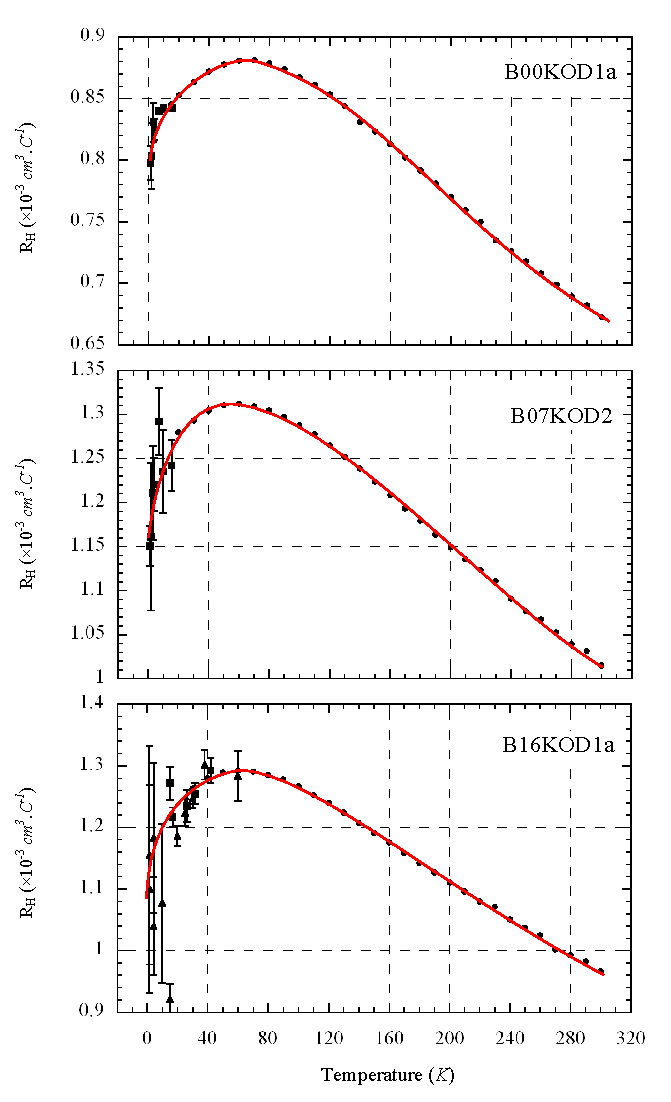
\includegraphics[scale=0.9]{Chapter-HallBSCO/Figures/HallIndividual/HallIndividualOD}
		\caption{$R_H$ for underdoped samples of \ac{BSCO}. Plots show results from, $\bullet$ Polo in June 2010, $\blacktriangle$ \ac{LNCMI} in June 2009, $\blacktriangledown$ \ac{LNCMI} in Feb 2010, $\blacksquare$ Nijmegen in May 2010. Symbols for comparable samples are marked on the plots. Red lines are a guide to the eye.}
		\label{Fig:ExpH:HallIndividualOD}
	\end{center}
\end{figure}

\begin{figure}[htbp]
	\begin{center}
		\includegraphics[scale=0.9]{Chapter-HallBSCO/Figures/HallIndividual/HallIndividualOP}
		\caption{$R_H$ for underdoped samples of \ac{BSCO}. Plots show results from, $\bullet$ Polo in June 2010, $\blacktriangle$ \ac{LNCMI} in June 2009, $\blacktriangledown$ \ac{LNCMI} in Feb 2010, $\blacksquare$ Nijmegen in May 2010. Symbols for comparable samples are marked on the plots. Dashed lines indicate points where the field was not sufficient to achieve linear behaviour. Red lines are a guide to the eye.}
		\label{Fig:ExpH:HallIndividualOP}
	\end{center}
\end{figure}

\begin{figure}[htbp]
	\begin{center}
		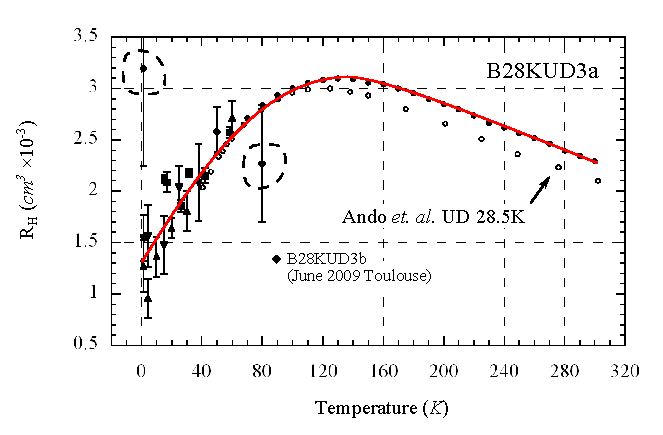
\includegraphics[scale=0.9]{Chapter-HallBSCO/Figures/HallIndividual/HallIndividualUD}
		\caption{$R_H$ for underdoped samples of \ac{BSCO}. Plots show results from, $\bullet$ Polo in June 2010, $\blacktriangle$ \ac{LNCMI} in June 2009, $\blacktriangledown$ \ac{LNCMI} in Feb 2010, $\blacksquare$ Nijmegen in May 2010. Symbols for comparable samples are marked on the plots. Dashed lines indicate points where the field was not sufficient to achieve linear behaviour. Red lines are a guide to the eye.}
		\label{Fig:ExpH:HallIndividualUD}
	\end{center}
\end{figure}
\begin{figure}[htbp]
	\begin{center}
		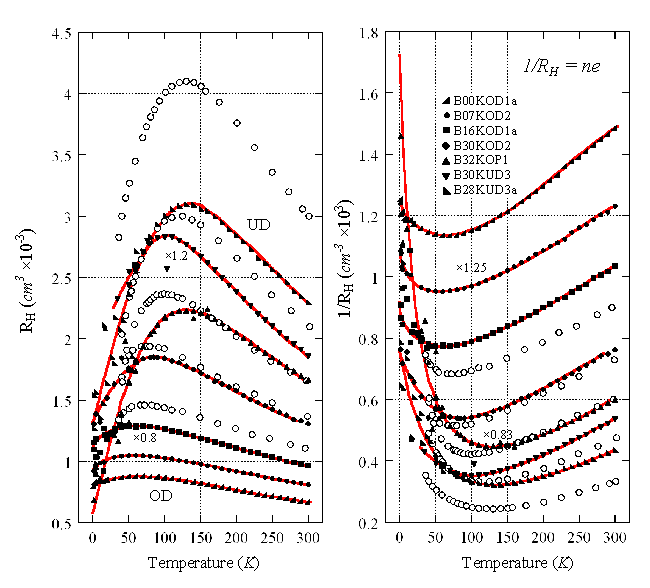
\includegraphics[scale=1.1]{Chapter-HallBSCO/Figures/InvHallCombined/InvHallCombined}
		\caption{Hall data in context with data from Ando \etal\cite{Ando1999} (open circles) which are in order of increasing $R_H$, 24KOD, 30KOD, 33KOP, 28.5KUD, 20KUD. Right panel shows the inverse hall data which relates to carrier density. Red lines are the same guides to the eye used in previous figures. Inset shows $R_H$ at \unit{300}{\kelvin} plus systematic error bars due primarily to uncertainty in thickness plus the necessary adjustments to follow the overal trend. B07KOD2, B32KOP1 and B30KUD3 have all been adjusted as detailed in the main text.}
		\label{Fig:ExpH:InvHallCombined}
	\end{center}
\end{figure}

With reference to figure~\ref{Fig:ExpH:InvHallCombined} and in particular the new low temperature data points, we see that doping strongly affects the qualitative shape of the $R_H$ curves. Whilst the trend appears to be that $R_H(\unit{300}{\kelvin})$ decreases as doping increases as to be expected, the $R_H(\unit{0}{\kelvin})$ values all tend toward approximately similar values of around \unit{$0.5\times 10^{-3}$}{\centi\metre\cubed}to \unit{$1.5\times 10^{-3}$}{\centi\metre\cubed}. The most proncounced diffreence between high and low temperature values though is with the optimally doped samples which are around $\times 2.75$ greater at high temperature.

There seems to be little evidence of the transition of the doping from $p$ to $1+p$ which agrees with the notion that these dopings lie beyond where the Fermi surface reconstruction is thought to take place~\cite{LeBoeuf2007}. 

%Divergence in resistivity occurs beyond UD 0K\cite{Ando2000}, well
%below our lowest nominal doping of ...

% Residual resistivity of ~20\mu\Ohm cm at optimal doping is very small
% and increases with La doping i.e. as become more underdoped
% \cite{Ando2000}


